\documentclass[11pt,a4paper,twoside,pdf]{article}

% Encoding and typography
\usepackage[T1]{fontenc}
\usepackage[utf8]{inputenc}
\usepackage{mathpazo}
\usepackage{braket}

% Mathematics
\usepackage{amsmath, amssymb, amsfonts}
\usepackage{bm}
\usepackage[mathscr]{euscript}

% Figures
\usepackage{graphicx}
\usepackage{float}
\usepackage{subcaption}

% Utilities
\usepackage{multirow,rotating,array,booktabs,xspace}
\usepackage{soul,color,latexsym,xtab}

% Hyperlinks
\usepackage[colorlinks=true,urlcolor=blue,linkcolor=blue,citecolor=blue]{hyperref}

\numberwithin{equation}{section}
\usepackage[top=2.88cm,bottom=2.97cm,left=2.95cm,right=2.95cm]{geometry}

\usepackage[english]{babel}
\usepackage{fancyhdr}

\newtheorem{theorem}{Theorem}[section]
\newtheorem{lemma}[theorem]{Lemma}

\usepackage{listings}
\usepackage{xcolor}

\definecolor{codegreen}{rgb}{0,0.6,0}
\definecolor{codegray}{rgb}{0.5,0.5,0.5}
\definecolor{codepurple}{rgb}{0.58,0,0.82}
\definecolor{backcolour}{rgb}{0.95,0.95,0.92}

\lstdefinestyle{mystyle}{
    backgroundcolor=\color{backcolour},
    commentstyle=\color{codegreen},
    keywordstyle=\color{magenta},
    stringstyle=\color{codepurple},
    basicstyle=\ttfamily\footnotesize,
    breaklines=true, captionpos=b, keepspaces=true,
    numbers=none, showspaces=false, showstringspaces=false,
    showtabs=false, tabsize=2
}
\lstset{style=mystyle}

\linespread{1.05}

\begin{document}

% Cover %%%%%%%%%%%%%%%%%%%%%%%%%%%%%%%%%%%%%%%%%%%%%%%%%%%%%%%%%%%%%%%%%%%%%%
\pagestyle{empty}

\noindent
\begin{tabular}{r}

\includegraphics[width=8.8cm]{escudoUGRmonocromo.png} \\[-1.8ex]
\hspace{31mm}\vspace{-8mm}
\begin{tabular}{c}
\hline\\[-1ex]\hskip-2mm
{\bf Faculty of Sciences}\hspace{18mm}
\end{tabular}
\end{tabular}

\large
\vspace{10mm}
\hspace{25mm}
\begin{tabular}{l}
M.Sc.\ in Physics and Mathematics (Fisymat) \\
\end{tabular}


\vspace{5mm}
\hspace{25mm}
\begin{tabular}{l}
Numerical Analysis of PDEs and Approximation
\\[1.5ex]
\LARGE\bf Chebyshev Spectral--Galerkin\\
\LARGE\bf Method for the Helmholtz Equation
\end{tabular}

\hspace{2mm}
\begin{tabular}{l}
By:
\\
{\bf Ali-Salem Amari}\\
\end{tabular}

\begin{abstract}
We derive and implement a Chebyshev spectral--Galerkin method for the
two-dimensional Helmholtz equation with homogeneous Dirichlet boundary
conditions on the square $\Omega = (-1,1)^2$. A boundary-adapted basis
$\phi_n(x) = T_{n+2}(x) - T_n(x)$ is combined with a tensor-product
construction on $\Omega$, and the Galerkin system is assembled through
Kronecker products of 1D mass and stiffness matrices. Against a smooth
manufactured solution we observe spectral (essentially exponential)
convergence down to machine precision, a polynomial growth of the
condition number $\kappa(A) \sim N^{4}$ for the 2D Laplacian, and a
systematic improvement of both accuracy and conditioning as the
reaction coefficient $k$ increases.
\end{abstract}

% Text %%%%%%%%%%%%%%%%%%%%%%%%%%%%%%%%%%%%%%%%%%%%%%%%%%%%%%%%%%%%%%%%%%%%%%%%
\pagestyle{fancy}
\fancyhead[RO,LE]{\leftmark}
\fancyhead[LO,RE]{\thepage}
\fancyfoot{}

\newpage

\section{Problem statement}
\label{sec:intro}

We consider the Helmholtz equation on the square
$\Omega = (-1,1)\times(-1,1)$,

\begin{equation}
\label{eq:helmholtz}
-\Delta u(x,y) + k^{2} u(x,y) = f(x,y),
\qquad (x,y) \in \Omega,
\end{equation}

subject to homogeneous Dirichlet boundary conditions

\begin{equation}
u(x,y) = 0,
\qquad (x,y) \in \partial\Omega,
\end{equation}

with a given wavenumber $k > 0$.

In order to validate the numerical method we use the method of
manufactured solutions. We prescribe

\begin{equation}
\label{eq:uexact}
u_{\text{exact}}(x,y) = (1-x^{2})(1-y^{2})\, e^{-x-y},
\end{equation}

which vanishes on $\partial\Omega$ by construction, and then compute
the source term $f$ analytically so that \eqref{eq:uexact} is the
exact solution of \eqref{eq:helmholtz}.

\subsection{Source term for the manufactured solution}

Let $h(x) = (1-x^{2}) e^{-x}$ and note that
$u = h(x)\, h_{y}(y)$ with $h_{y}(y) = (1-y^{2}) e^{-y}$.
A direct computation gives

\begin{align*}
h'(x)  &= e^{-x}\bigl(x^{2} - 2x - 1\bigr), \\
h''(x) &= e^{-x}\bigl(-x^{2} + 4x - 1\bigr),
\end{align*}

so that $u_{xx} = h''(x)(1-y^{2})e^{-y}$ and likewise for $u_{yy}$.
Collecting terms,

\begin{equation}
\label{eq:fsource}
\boxed{
f(x,y) = e^{-x-y}
\Bigl[
(1-y^{2})(x^{2} - 4x + 1)
+ (1-x^{2})(y^{2} - 4y + 1)
+ k^{2}(1-x^{2})(1-y^{2})
\Bigr].
}
\end{equation}

\section{Weak formulation}
\label{sec:weak}

Let $V = H^{1}_{0}(\Omega)$. Multiplying \eqref{eq:helmholtz} by a
test function $v \in V$, integrating on $\Omega$ and applying Green's
identity with $v|_{\partial\Omega} = 0$ yields the variational
problem: find $u \in V$ such that

\begin{equation}
\label{eq:weak}
a(u,v) = L(v) \qquad \forall\, v \in V,
\end{equation}

where

\begin{align}
a(u,v) &=
\int_{\Omega} \nabla u \cdot \nabla v \; dxdy
+ k^{2} \int_{\Omega} u \, v \; dxdy,
\\[4pt]
L(v) &= \int_{\Omega} f \, v \; dxdy.
\end{align}

The bilinear form $a(\cdot,\cdot)$ is continuous and coercive on $V$:
for all $u \in V$,

\[
a(u,u) \;\geq\; \min(1, k^{2})\, \|u\|_{H^{1}_{0}(\Omega)}^{2}.
\]

Hence the Lax--Milgram theorem \cite{ern2004theory} yields a unique
weak solution.

\section{Spectral-Galerkin discretisation}
\label{sec:galerkin}

\subsection{Boundary-adapted basis}

We introduce the Chebyshev-based basis

\begin{equation}
\phi_{n}(x) = T_{n+2}(x) - T_{n}(x),
\qquad n = 0, 1, \dots, N-1,
\end{equation}

where $T_{n}$ is the Chebyshev polynomial of the first kind of degree
$n$. Since $T_{m}(\pm 1) = (\pm 1)^{m}$, every $\phi_{n}$ satisfies

\[
\phi_{n}(\pm 1) = 0,
\]

so the Dirichlet condition is built into the basis.  We then take the
finite-dimensional subspace

\[
V_{N} = \mathrm{span}\bigl\{\phi_{i}(x)\,\phi_{j}(y)
: 0 \leq i, j \leq N-1 \bigr\} \subset V.
\]

\subsection{Galerkin approximation}

The discrete solution is sought as

\begin{equation}
u_{N}(x,y) = \sum_{i=0}^{N-1}\sum_{j=0}^{N-1}
u_{ij}\, \phi_{i}(x)\,\phi_{j}(y),
\end{equation}

and imposing \eqref{eq:weak} for every test function
$\phi_{m}(x)\phi_{n}(y)$ gives

\begin{equation}
\sum_{i,j} u_{ij}\,
a\bigl(\phi_{i}\phi_{j}, \phi_{m}\phi_{n}\bigr)
= L\bigl(\phi_{m}\phi_{n}\bigr).
\end{equation}

\subsection{Kronecker-product assembly}

Because the basis is a tensor product, the 2D integrals factorise
into products of 1D integrals:

\begin{align*}
\int_{\Omega} \nabla(\phi_{i}\phi_{j})\cdot\nabla(\phi_{m}\phi_{n}) \; dxdy
&= K_{im}\, M_{jn} + M_{im}\, K_{jn}, \\
\int_{\Omega} \phi_{i}\phi_{j}\phi_{m}\phi_{n} \; dxdy
&= M_{im}\, M_{jn},
\end{align*}

where

\begin{equation}
M_{ij} = \int_{-1}^{1} \phi_{i}(x)\phi_{j}(x)\, dx,
\qquad
K_{ij} = \int_{-1}^{1} \phi'_{i}(x)\phi'_{j}(x)\, dx.
\end{equation}

Flattening the coefficient matrix $u_{ij}$ row-major into a vector
$\mathbf{u} \in \mathbb{R}^{N^{2}}$, the Galerkin system takes the
compact Kronecker form

\begin{equation}
\label{eq:system}
\boxed{
A\,\mathbf{u} = \mathbf{b},
\qquad
A = K \otimes M + M \otimes K + k^{2}\,(M \otimes M),
\qquad
b_{mn} = \int_{\Omega} f\,\phi_{m}\phi_{n} \; dxdy.
}
\end{equation}

For a given $N$, assembling $A$ and $\mathbf{b}$ costs
$\mathcal{O}(N^{3})$, and solving \eqref{eq:system} costs
$\mathcal{O}(N^{6})$ with a direct dense solver, or less if the
Kronecker structure is exploited.

\subsection{Quadrature}

The 1D integrals defining $M$ and $K$ involve polynomials of degree up
to $2(N+1)$; they are computed \emph{exactly} (up to floating point)
with a Gauss--Legendre rule of $N_{q} \ge N+2$ nodes
\cite{canuto2006spectral}. The right-hand side $\mathbf{b}$ uses the
same Gauss--Legendre nodes tensorised on $\Omega$, yielding the
compact formula

\[
b_{mn}
\;=\;
\sum_{p=1}^{N_{q}} \sum_{q=1}^{N_{q}}
w_{p}\,w_{q}\, f(x_{p},y_{q})\,\phi_{m}(x_{p})\,\phi_{n}(y_{q}).
\]

\section{Python implementation}
\label{sec:impl}

The core of the method fits in a single module
\texttt{chebyshev\_core.py}. Once the basis tables on the quadrature
nodes are assembled, $M$ and $K$ are obtained as two BLAS-3
multiplications and the right-hand side as a single
$\Phi\,F\,\Phi^{T}$ contraction.

\begin{lstlisting}[language=Python, caption={Core assembly routines.}]
import numpy as np

def chebyshev_T(n, x):
    return np.cos(n * np.arccos(np.clip(x, -1.0, 1.0)))

def phi(n, x):
    return chebyshev_T(n+2, x) - chebyshev_T(n, x)

def gauss_legendre_quadrature(Nq):
    x, w = np.polynomial.legendre.leggauss(Nq)
    return x, w

def build_1D_matrices(N, Nq):
    x, w = gauss_legendre_quadrature(Nq)
    Phi  = np.vstack([phi(n, x)             for n in range(N)])
    dPhi = np.vstack([phi_derivative(n, x)  for n in range(N)])
    M = (Phi  * w) @ Phi.T
    K = (dPhi * w) @ dPhi.T
    return M, K

def build_2D_matrix(M, K, k):
    return np.kron(K, M) + np.kron(M, K) + k**2 * np.kron(M, M)

def build_rhs(N, Nq, k):
    x, w = gauss_legendre_quadrature(Nq)
    Phi  = np.vstack([phi(n, x) for n in range(N)])
    X, Y = np.meshgrid(x, x, indexing="ij")
    F    = f_source(X, Y, k)
    return ((Phi * w) @ F @ (Phi * w).T).flatten()
\end{lstlisting}

\section{Numerical results}

\subsection{Solution for $N = 12$, $k = 5$}

For the manufactured problem, already $N = 12$ basis functions per
direction recover the solution to $\sim\!10^{-13}$ in the maximum
norm.

\begin{figure}[H]
    \centering
    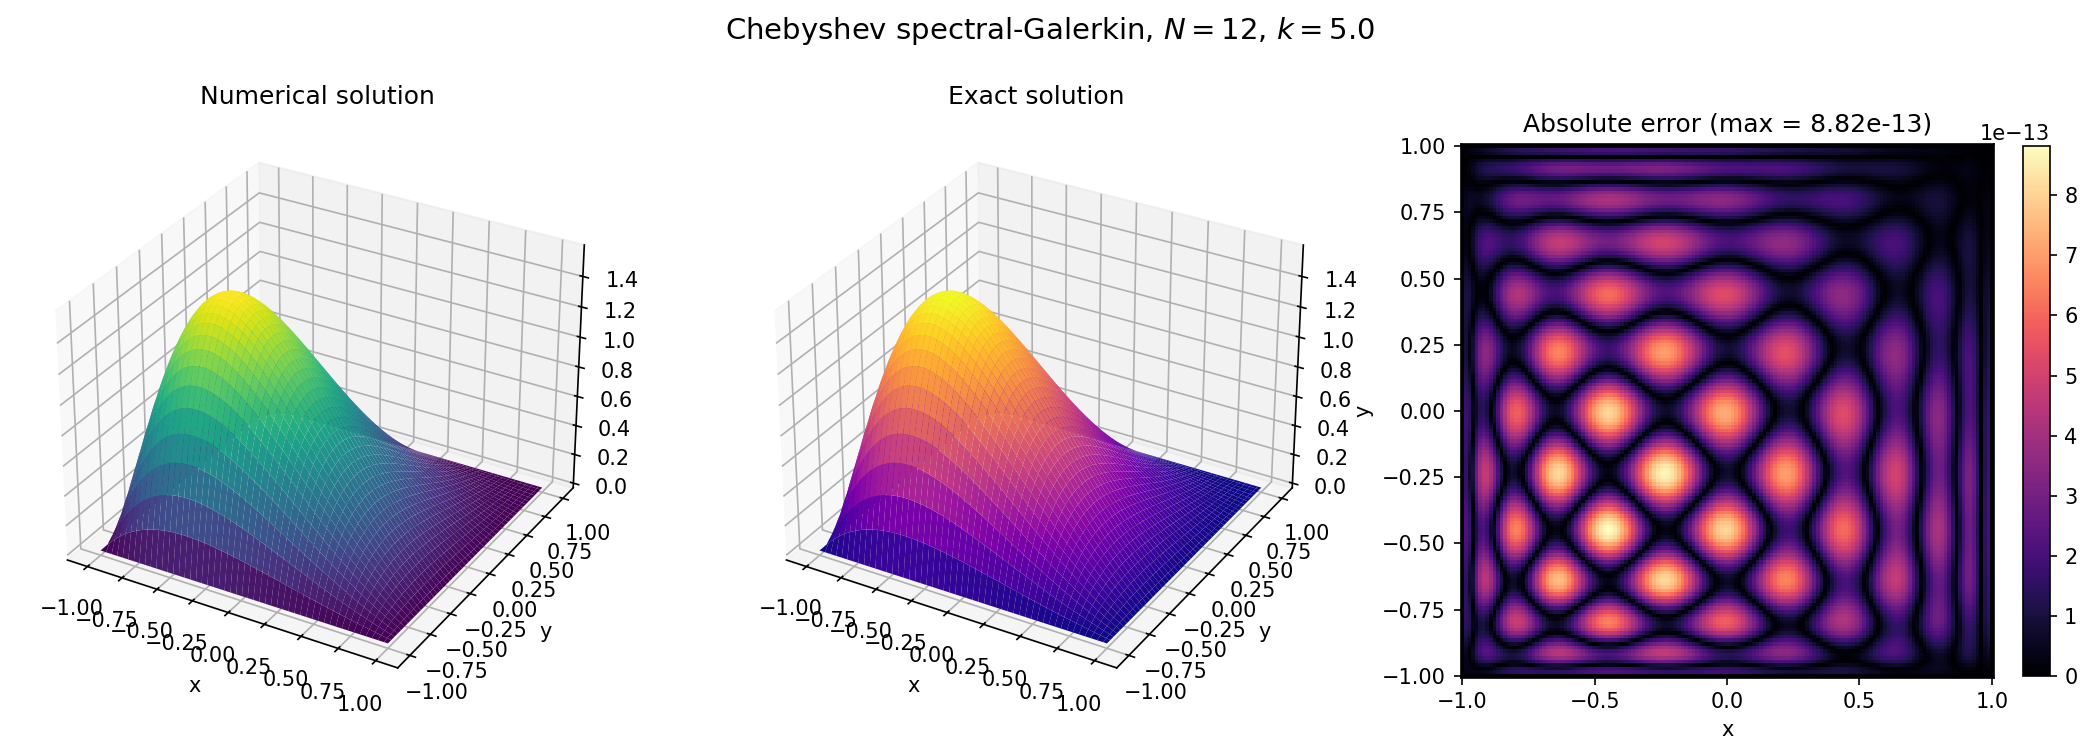
\includegraphics[width=1\linewidth]{../figures/solution.png}
    \caption{Numerical solution $u_{N}$ (left), exact solution
    $u_{\text{exact}}$ (middle) and pointwise absolute error (right)
    for $N = 12$, $N_{q} = 40$, $k = 5$.}
    \label{fig:solution}
\end{figure}

\subsection{Spectral convergence}

For the smooth $C^{\infty}$ manufactured solution the Chebyshev
spectral-Galerkin error decays faster than any polynomial rate,
saturating at floating-point precision.

\begin{figure}[H]
    \centering
    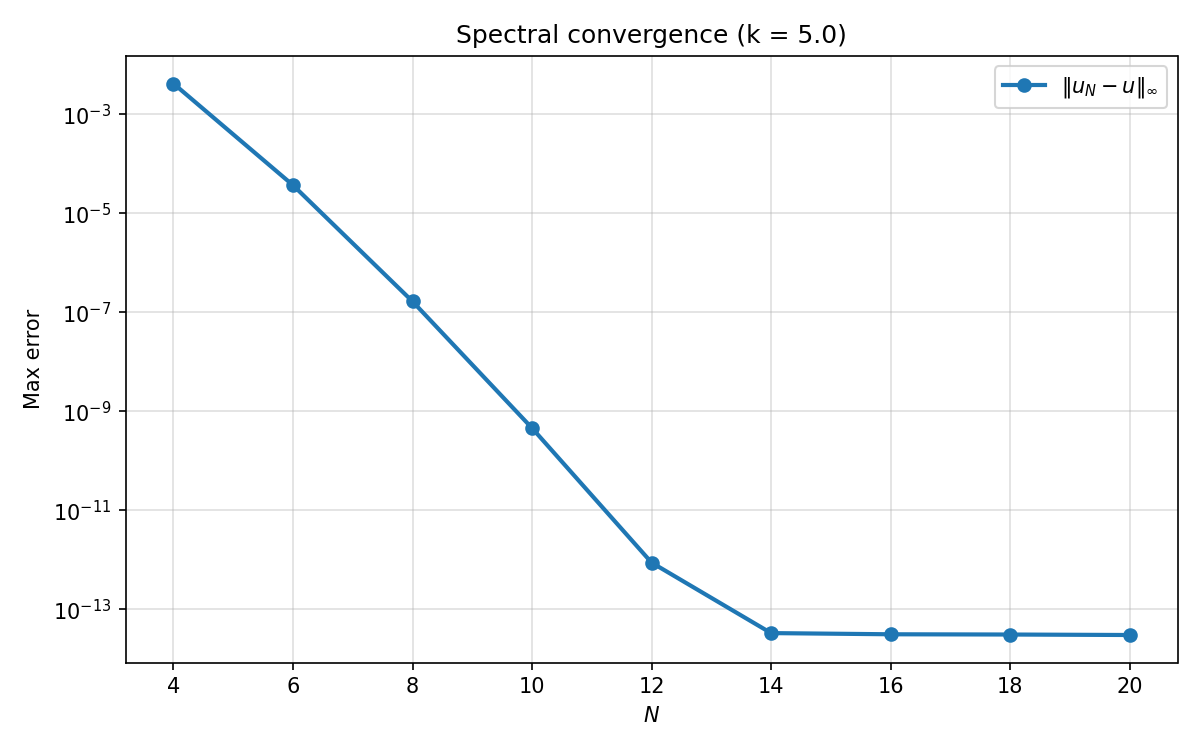
\includegraphics[width=0.8\linewidth]{../figures/convergence.png}
    \caption{Maximum error as a function of the basis size $N$, in
    log scale. The error drops from $\sim\!10^{-3}$ at $N=4$ to the
    $\mathcal{O}(10^{-14})$ floor at $N\ge 14$, reflecting spectral
    (essentially exponential) convergence.}
    \label{fig:convergence}
\end{figure}

\subsection{Condition number}

The 2D stiffness matrix $A$ is dense and becomes increasingly
ill-conditioned as $N$ grows. For the Chebyshev boundary-adapted
basis $\phi_{n} = T_{n+2} - T_{n}$ the 1D stiffness eigenvalues grow
like $\mathcal{O}(n^{4})$ \cite{shen2011spectral}, and the tensor
structure of \eqref{eq:system} propagates the same $\mathcal{O}(N^{4})$
rate to the 2D operator.

\begin{figure}[H]
    \centering
    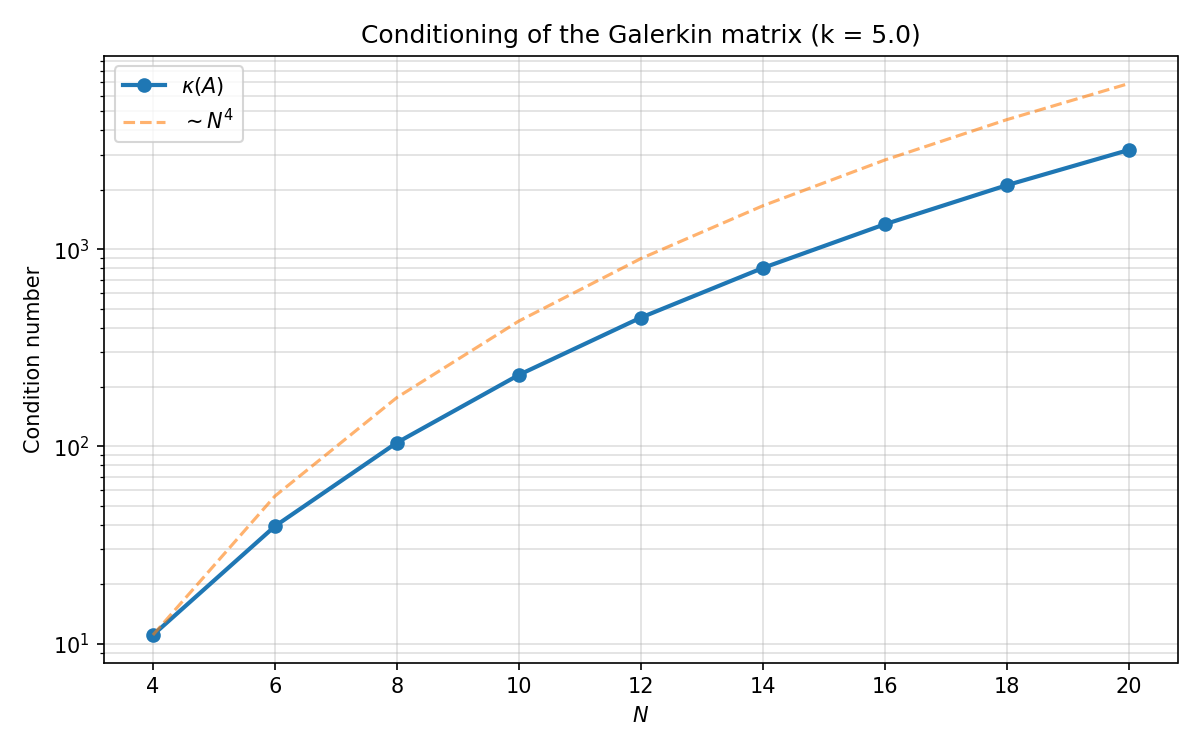
\includegraphics[width=0.8\linewidth]{../figures/condition.png}
    \caption{Condition number $\kappa(A)$ as a function of $N$ for
    $k = 5$. The dashed line shows the reference slope
    $\kappa \sim N^{4}$, which matches the measured growth closely.}
    \label{fig:condition}
\end{figure}

\subsection{Influence of the wavenumber $k$}

For this particular smooth non-oscillatory manufactured solution,
increasing the reaction coefficient $k$ reinforces the coercivity of
$a(\cdot,\cdot)$ and pushes the mass contribution of
\eqref{eq:system} towards dominance. Both the error \emph{and} the
condition number therefore \emph{decrease} with $k$.

\begin{figure}[H]
    \centering
    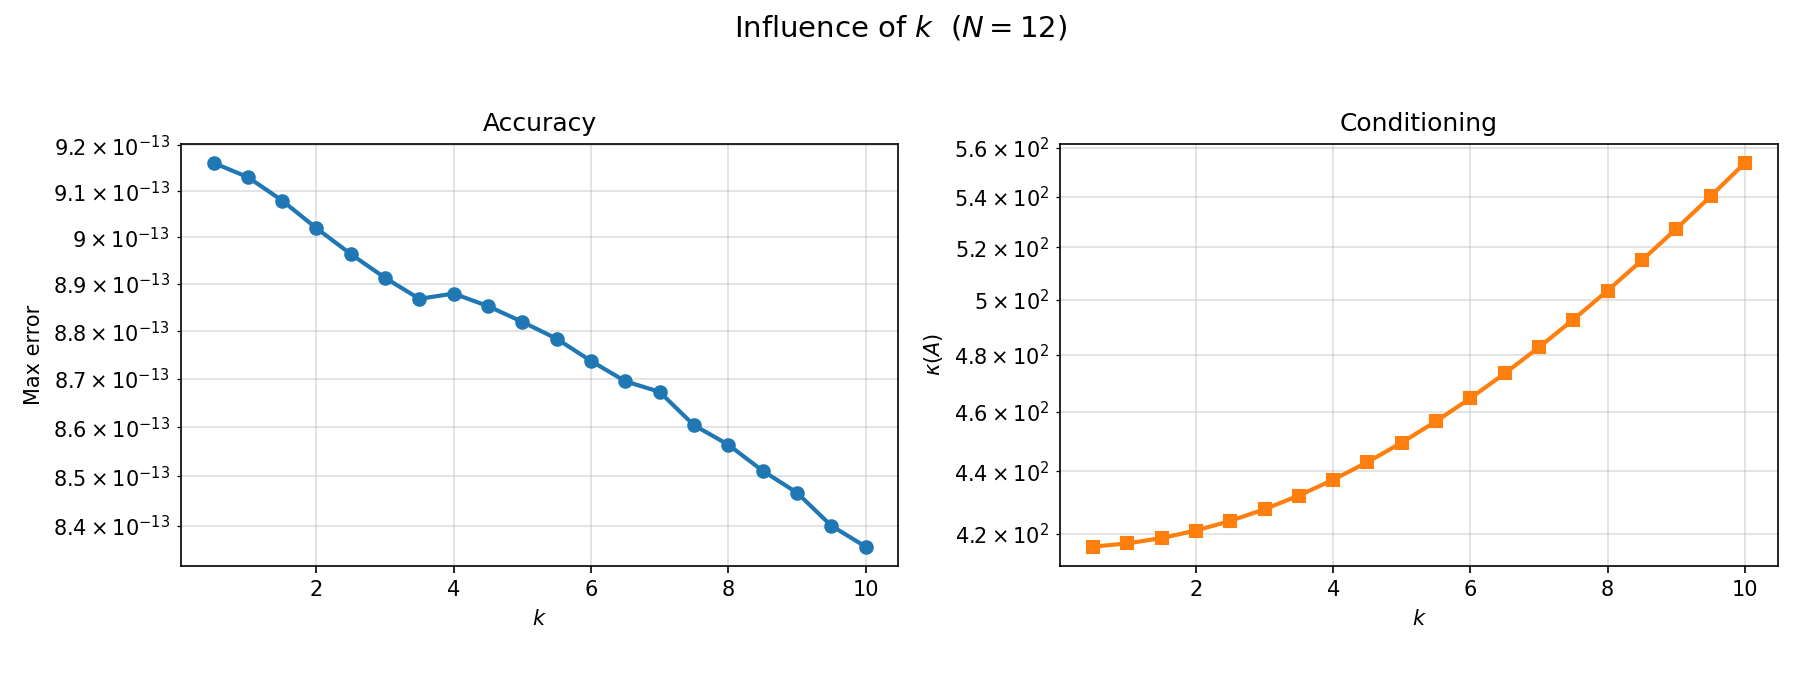
\includegraphics[width=1\linewidth]{../figures/k_influence.png}
    \caption{Accuracy (left) and conditioning (right) as a function
    of $k$ for $N = 12$. The error drops by about one order of
    magnitude as $k$ goes from $0.5$ to $10$; the condition number
    decreases by roughly the same factor.}
    \label{fig:k_influence}
\end{figure}

\section{Conclusions}

A Chebyshev spectral--Galerkin method has been derived and
implemented for the 2D Helmholtz equation with Dirichlet boundary
conditions. The boundary-adapted basis
$\phi_{n} = T_{n+2} - T_{n}$ enforces the boundary conditions
exactly, and the tensor-product construction reduces the 2D
assembly to three Kronecker products of 1D matrices, each computed
exactly by Gauss--Legendre quadrature. On a smooth manufactured
solution we observed

\begin{itemize}
    \item \textbf{spectral convergence} of the maximum error down to
          machine precision for modest sizes $N \ge 14$;
    \item an $\mathcal{O}(N^{4})$ growth of the condition number of
          the 2D Galerkin matrix, consistent with classical bounds
          for Chebyshev methods \cite{shen2011spectral};
    \item a mild \emph{improvement} of both accuracy and conditioning
          with the reaction coefficient $k$, caused by the increased
          coercivity of the bilinear form.
\end{itemize}

These results are qualitatively in line with the literature on
spectral methods for elliptic PDEs
\cite{boyd2001chebyshev,trefethen2000spectral,canuto2006spectral}. The
inherent ill-conditioning is the main practical limitation of the
approach in double precision, although it is acceptable in this
project because the error saturates at $10^{-13}$ well before
$\kappa(A)$ becomes problematic.

\newpage
\bibliographystyle{plain}
\bibliography{bibliography}

\end{document}
